%%%%%%%%%%%%%%%%%%%%%%%%%%%%%%%%%%%%%%%%%%%%%%%%%%%%%%%%%%%%%%%%%%%%%%%%%%%%%%%
% Chapter 2: Fundamentos Te�ricos 
%%%%%%%%%%%%%%%%%%%%%%%%%%%%%%%%%%%%%%%%%%%%%%%%%%%%%%%%%%%%%%%%%%%%%%%%%%%%%%%

%++++++++++++++++++++++++++++++++++++++++++++++++++++++++++++++++++++++++++++++

El m�todo de la bisecci�n se basa en dos teoremas, el de Bolzano y el del Valor Intermedio que explicaremos a continuaci�n, y es empleado para aproximar ceros de funciones.

Supongamos que queremos encontrar las ra�ces de una funci�n $f(x)$ continua. Dados dos puntos a y b, tal que $f(a)$ y $f(b)$ tengan signos distintos, sabemos por el Teorema de Bolzano que $f(x)$ debe tener, al menos, una ra�z en el intervalo [a,b]. Este m�todo divide el intervalo en dos utilizando un tercer punto c= $\frac{a+b}{2}$. De esta forma, se dar�n dos posibilidades: $f(a)$ y $f(c)$, � $f(c)$ y $f(b)$ tienen distinto signo. Se aplica este m�todo al subintervalo donde ocurre el cambio de signo. As� se realizar� tantas vecse como sea necesario para conseguir la m�xima precisi�n.
%++++++++++++++++++++++++++++++++++++++++++++++++++++++++++++++++++++++++++++++

\section{Teorema de Bolzano}
\label{2:sec:1}
Sea $f(x)$ una funci�n continua en un intervalo [a,b] tal que $f(a)*f(b)<0$, entonces existe un punto c perteneciente al intervalo (a,b) tal que $f(c)=0$
\subsection{Demostraci�n Teorema de Bolzano}
\label{2:sec:1:sec:1}
Supongamos que $f(a)<0$ y $f(b)>0$. Sea A el conjunto formado por todos los valores x tal que x pertenece al intervalo [a,b] para los que $f(x)<0$. El conjunto A est� acotado superiormente por b, y adem�s, no es vaci� ya que a pertenece a A. Por ello el conjunto A tiene un extremo superior c. Se cumple que $f(c)=0$. Ve�moslo:

Si $f(c)>0$, entonces por la propiedad de la conservaci�n del signo de las funciones continuas existir�a un intervalo $(c-\alpha, c+\alpha)$ en el que la funci�n ser�a tambi�n positiva. En este caso existir�an valores menores que c que servir�an de cota superior de A y por ello c no ser�a el extremo superior de A como hemos supuesto. 

Si $f(c)<0$, entonces existir�a un intervalo $(c-\alpha, c+\alpha)$ en el que la funci�n ser�a negativa y por tanto exist�an valores de x a la derecha de c para los que la funci�n ser�a negativa y por tanto c no ser�a extremo superior de A. De este modo, $f(c)$ tiene que tomar el valor cero: $f(c)=0$.

\section{Teorema del Valor Intermedio}
\label{2:sec:2}
Sea $f(x)$ una funci�n continua en un intervalo [a,b], tal que $f(a)<f(b)$ entonces, para todo k tal que $f(a)<k<f(b)$ existe $x_0$ que pertenece al intervalo (a,b) tal que $f(x_0)=k$.
\subsection{Demostraci�n Teorema del Valor Intermedio}
\label{2:sec:2:sec:1}
 Para la demostraci�n aplicamos el Teorema de Bolzano en la funci�n $g(x)=f(x)-k$, la cual es continua por serlo $f(x)$, $g(a)<0$ y $g(b)>0$. El teorema nos permite afirmar que existir� un c perteneciente al intervalo (a,b) tal que $g(c)=0$ y en consecuencia $f(c)=k$.
\section{Gr�fica}
En esta gr�fica reflejamos los resultados te�ricos esperados tras realizar los experimentos propuestos en el siguiente cap�tulo. Podemos observar como la funci�n $f(x)=5^x-5$ tiene una ra�z en el punto $(1,0)$.

\includegraphics[scale=0.50]{grafcap2.eps}

